\begin{frame}
  \frametitle{RRM for short-term dependability}
  
  \begin{itemize}
  \item Issue:  Dependable communication 
    \begin{itemize}
    \item over fading channels 
    \item with short deadlines 
    \item and limited  diversity
    \item but with some limited prediction (deadline longer than
      coherence time) 
    \end{itemize}
  \item Bad combination -- but what is achievable? 
  \end{itemize}
\end{frame}

\begin{frame}
  \frametitle{First approach: Markov model for fading channel}

  \begin{itemize}
  \item Markov chain extracted from  Clark's model 
    \begin{itemize}
    \item States correspond to SNR regions
    \item which in turn correspond to
      Modulation/Coding Scheme (MCS) performance at acceptable error rate 
    \end{itemize}
  \item Under these assumption: 
    \begin{itemize}
    \item What is the \emph{time-limited capacity}, for an acceptable
      error probability?
      \begin{itemize}
      \item In a sense: Real-time version of outage capacity 
      \end{itemize}
    \item Can it be communicated to a control system as options? 
    \end{itemize}
  \item Formulate as Markov reward model 
  \end{itemize}
\end{frame}

\begin{frame}
  \frametitle{Time-limited capacity: Influencing factors}
  \begin{center}
    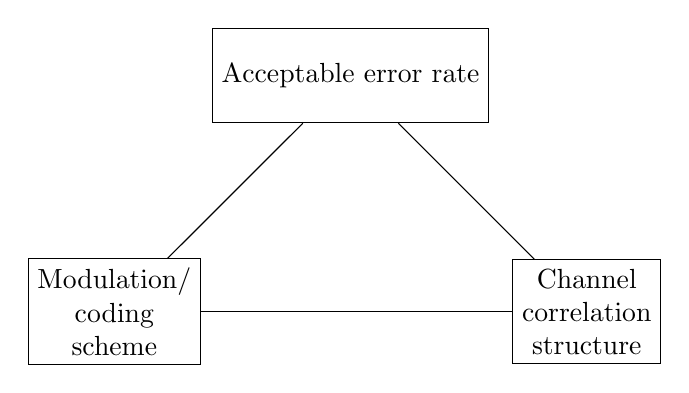
\begin{tikzpicture}[box/.style = {draw, minimum height=12mm,
        align=center}]
      \node (aer) [box] at (3,3) {Acceptable error rate}; 
      \node (mcs) [box] at (0,0)  {Modulation/\\coding\\scheme}; 
      \node (ccs) [box] at (6,0)  {Channel \\correlation\\ structure}; 
      \draw[] (aer) -- (mcs); 
      \draw[] (aer) -- (ccs); 
      \draw[] (mcs) -- (ccs); 
    \end{tikzpicture}
  \end{center}
\end{frame}

\begin{frame}
  \frametitle{Time-limited capacity: First hints at results}
  \begin{itemize}
    
  \item Over increasing number of time slots 
  \item What is the (normalized, per time slot) available capacity
  \item For different acceptable error rates 
  \item \textbf{Observation}: Rate of increase depends on acceptable error rate 
  \end{itemize}
  
  \begin{center}
    \includegraphics[width=0.6\columnwidth]{rewards-correlated}
  \end{center}

\end{frame}


% \begin{frame}
%   \frametitle{}
% \end{frame}

%%% Local Variables:
%%% mode: latex
%%% TeX-master: "presentation_1"
%%% End:
